%\documentclass[12pt]{article}

\questionheader{ex:s3.1}


%%%%%%%%%%%%%%%%%%
\subsection*{\Conceptual}
%%%%%%%%%%%%%%%%%%

%%%%%%%%%%%%%%%%%%%%%%%%%%%%
%\Instructions{Questions~\ref{prob_s1.0first} through \ref{prob_s1.0last} provide practice with.}
%%%%%%%%%%%%%%%%%%%%

%%%%%%%%%%%%%%%%%%%%%%%%%%%%%%%%
\begin{question}
For each of the following, evaluate the given double integral 
\emph{without} using iteration. Instead, interpret the integral as, for
example, an area or a volume.
\begin{enumerate}[(a)]
\item
$\dst\int_{-1}^3\int_{-4}^1 \dee{y}\,\dee{x}$
\item
$\dst\int_0^2\int_0^{\sqrt{4-y^2}} \dee{x}\,\dee{y}$
\item
$\dst\int_{-3}^3\int_0^{\sqrt{9-y^2}}\sqrt{9-x^2-y^2}\ \dee{x}\,\dee{y}$
\end{enumerate}
\end{question}

%\begin{hint}
%
%\end{hint}

\begin{answer}
(a) $20$\qquad
(b) $\pi$  \qquad
(c) $9\pi$
\end{answer}

\begin{solution}
(a) The given double integral
$\int_{-1}^3\int_{-4}^1 \dee{y}\,\dee{x}=\dblInt_R \dee{x}\,\dee{y}$ 
where
\begin{equation*}
R=\Set{(x,y)}{ -1\le x\le 3,\ -4\le y\le1}
\end{equation*}
and so the integral is the area of a rectangle with sides of lengths 
$4$ and $5$.  Thus $\int_{-1}^3\int_{-4}^1 \dee{y}\,\dee{x}=4\times 5=20$.

(b) The given double integral
$\dst\int_0^2\int_0^{\sqrt{4-y^2}} \dee{x}\,\dee{y}
     =\dst\dblInt_R \dee{x}\,\dee{y}$ 
where
\begin{align*}
R&=\Set{(x,y)}{ 0\le y\le 2,\ 0\le x\le\sqrt{4-y^2}} \\
&=\Set{(x,y)}{ x\ge 0,\ y\ge 0,\ y\le 2,\ x^2+y^2\le 4} 
\end{align*}
So $R$ is the first quadrant part of the circular disk of radius $2$
centred on $(0,0)$. The area of the full disk is $\pi\,2^2=4\pi$. 
The given integral is one quarter of that, which is $\pi$.

(c) The given double integral
$\dst\int_{-3}^3\int_0^{\sqrt{9-y^2}}\sqrt{9-x^2-y^2}\ \dee{x}\,\dee{y}
     =\dst\dblInt_{\cR} z(x,y)\ \dee{x}\,\dee{y}$ 
where $z(x,y)=\sqrt{9-x^2-y^2}$ and
\begin{align*}
\cR&=\Set{(x,y)}{ -3\le y\le 3,\ 0\le x\le\sqrt{9-y^2}} \\
&=\Set{(x,y)}{ x\ge 0,\ -3\le y\le 3,\ \ x^2+y^2\le 9} 
\end{align*}
So $\cR$ is the right half of the circular disk of radius $3$
centred on $(0,0)$. By Equation (\eref{CLP200}{eqn Volume y slice}) 
in the CLP-3 text, the given integral is the volume of the solid
\begin{align*}
\cV&=\Big\{\,(x,y,z)\,\Big|\,(x,y)\in\cR,\ 0\le z\le \sqrt{9-x^2-y^2}\,\Big\}\\
&=\Big\{\,(x,y,z)\,\Big|\,(x,y)\in\cR,\ z\ge 0,\ x^2+y^2+z^2\le 9\,\Big\}
\end{align*}
Thus $\cV$ is the one quarter of the spherical ball of radius $3$ and 
centre $(0,0,0)$ with $x\ge 0$ and $z\ge 0$. So
\begin{equation*}
\int_{-3}^3\int_0^{\sqrt{9-y^2}}\sqrt{9-x^2-y^2}\ \dee{x}\,\dee{y}
=\frac{1}{4}\Big(\frac{4}{3}\pi 3^3\Big)
=9\pi
\end{equation*} 




\end{solution}


%%%%%%%%%%%%%%%%%%%%%%%%%%%%%%%%
\begin{question}
Let $f(x,y)= 12 x^2y^3$. Evaluate
\begin{enumerate}[(a)]
\item
$\dst\int_0^3 f(x,y)\,\dee{x}$
\item
$\dst\int_0^2 f(x,y)\,\dee{y}$
\item
$\dst\int_0^2\int_0^3 f(x,y)\,\dee{x}\,\dee{y}$
\item
$\dst\int_0^3\int_0^2 f(x,y)\,\dee{y}\,\dee{x}$
\item
$\dst\int_0^3\int_0^2 f(x,y)\,\dee{x}\,\dee{y}$
\end{enumerate}
\end{question}

\begin{hint}
Be careful to match each integration variable with its own limits.
Remember that the integral with respect to $x$ treats $y$ as a constant and 
the integral with respect to $y$ treats $x$ as a constant.
\end{hint}

\begin{answer}
(a) $108 y^3$\qquad
(b) $48x^2$\qquad
(c), (d) $432$\qquad
(e) $648$
\end{answer}

\begin{solution}
(a) The integral with respect to $x$ treats $y$ as a constant. So
\begin{align*}
\int_0^3 f(x,y)\,\dee{x}
  &= \int_0^3 12 x^2y^3\,\dee{x}
   = \Big[4x^3y^3\Big]_{x=0}^{x=3}
   = 108 y^3
\end{align*}

(b) The integral with respect to $y$ treats $x$ as a constant. So
\begin{align*}
\int_0^2 f(x,y)\,\dee{y}
  &= \int_0^2 12 x^2y^3\,\dee{y}
   = \Big[3x^2y^4\Big]_{y=0}^{y=2}
   = 48x^2
\end{align*}

(c) By part (a)
\begin{align*}
\int_0^2\int_0^3 f(x,y)\,\dee{x}\,\dee{y}
&=\int_0^2\left[\int_0^3 f(x,y)\,\dee{x}\right]\dee{y}
 =\int_0^2 108y^3\,\dee{y}
 =\Big[27y^4\Big]_{y=0}^{y=2} \\
&=27\times 16 
= 432
\end{align*}

(d) By part (b)
\begin{align*}
\int_0^3\int_0^2 f(x,y)\,\dee{y}\,\dee{x}
&=\int_0^3\left[\int_0^2 f(x,y)\,\dee{y}\right]\dee{x}
 =\int_0^3 48x^2\,\dee{y}
 =\Big[16x^3\Big]_{x=0}^{x=3} \\
&=16\times 27 
= 432
\end{align*}

(e) This time
\begin{align*}
\int_0^3\int_0^2 f(x,y)\,\dee{x}\,\dee{y}
&=\int_0^3\left[\int_0^2 12 x^2y^3\,\dee{x}\right]\dee{y}
=\int_0^3\left[4 x^3y^3\right]_0^2\dee{y}
=\int_0^3 32 y^3\dee{y} \\
& =\Big[8y^4\Big]_0^3 
 =8\times 81
 = 648
\end{align*}

\end{solution}


%%%%%%%%%%%%%%%%%%
\subsection*{\Procedural}
%%%%%%%%%%%%%%%%%%

%%%%%%%%%%%%%%%%%%%%%%%%%%%%
\Instructions{Questions~\ref{prob_s3.1a} through \ref{prob_s3.1f} provide practice with limits of integration for double integrals in Cartesian coordinates.}
%%%%%%%%%%%%%%%%%%%%

%%%%%%%%%%%%%%%%%%%%%%%%%%%%%%%%
\begin{question} \label{prob_s3.1a}
For each of the following, evaluate the given double integral 
\emph{using} iteration.
\begin{enumerate}[(a)]
\item 
$\displaystyle\dblInt_R (x^2+y^2)\,\dee{x}\,\dee{y}$ where $R$ is the rectangle 
$0\le x\le a,\ 0\le y\le b$ where $a>0$ and $b>0$.
\item
$\displaystyle\dblInt_T (x-3y)\,\dee{x}\,\dee{y}$ where $T$ is the triangle 
with vertices $(0,0),\ (a,0),\ (0,b)$.
\item
$\displaystyle\dblInt_R xy^2\,\dee{x}\,\dee{y}$ where $R$ is the finite 
region in the first quadrant bounded by the curves $y=x^2$ and $x=y^2$.
\item 
$\displaystyle\dblInt_D x\cos y\,\dee{x}\,\dee{y}$ where $D$ is 
the finite region in the first quadrant bounded by the coordinate axes 
and the curve $y=1-x^2$.
\item
$\displaystyle\dblInt_R {x\over y}e^y\,\dee{x}\,\dee{y}$ where $R$ is 
the region $0\le x\le 1,\ x^2\le y\le x$.
\item
$\displaystyle\dblInt_T {xy\over 1+x^4}\,\dee{x}\,\dee{y}$  where $T$ 
is the triangle with vertices $(0,0),\ (0,1),\ (1,1)$.
\end{enumerate}
\end{question}

%\begin{hint}
%
%\end{hint}

\begin{answer}
(a) $\frac{1}{3}\big(a^3b+ab^3\big)$ \qquad
(b) $\frac{a^2b}{6}-\frac{ab^2}{2}$  \qquad
(c) $\frac{3}{56}$ \qquad
(d) $\frac{1}{2}(1-\cos 1)$ \qquad
(e) $\frac{1}{2}(e-2)$  

(f) $\frac{1}{4}\left(\frac{\pi}{4}-\frac{1}{2}\ln 2\right)$ 
\end{answer}

\begin{solution}
The following figures show the domains of integration for the
integrals in this problem.
\begin{center}
  (a) \raisebox{-0.5\height}{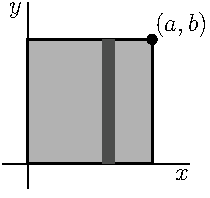
\includegraphics{domain2a.pdf}}\qquad
  (b) \raisebox{-0.5\height}{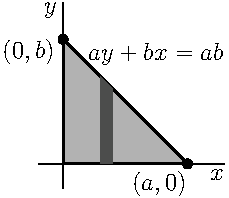
\includegraphics{domain2b.pdf}}\qquad
  (c) \raisebox{-0.5\height}{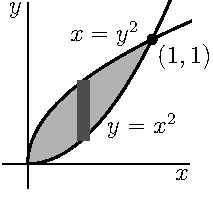
\includegraphics{domain2c.pdf}}            
\end{center}
\begin{center}
  (d) \raisebox{-0.5\height}{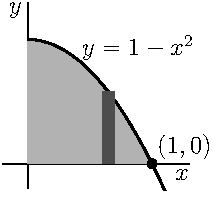
\includegraphics{domain2d.pdf}}\qquad
  (e) \raisebox{-0.5\height}{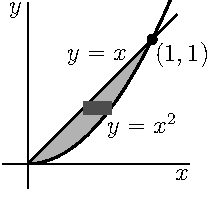
\includegraphics{domain2e.pdf}}\qquad
  (f) \raisebox{-0.5\height}{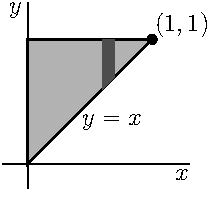
\includegraphics{domain2f.pdf}}
\end{center}

\leqnomode
\begin{align*}
\dblInt_R (x^2+y^2)\,\dee{x}\,\dee{y}
&=\int_0^a \dee{x}\int_0^b\dee{y}\ (x^2+y^2)
=\int_0^a \dee{x}\,\left(x^2b+\frac{1}{3}b^3\right)
\tag{a} \\
&=\frac{1}{3}\big(a^3b+ab^3\big)
\notag \displaybreak[0]\\
\noalign{\smallskip}
%%%
\dblInt_T (x-3y)\,\dee{x}\,\dee{y}
&=\int_0^a \dee{x}\int_0^{b(1-{x\over a})}\dee{y}\,(x-3y)
\tag{b} \\
&=\int_0^a \dee{x}\,\left[bx\left(1-\frac{x}{a}\right)
     -\frac{3}{2}b^2\left(1-\frac{x}{a}\right)^2\right]
\notag \\
&=\left[\frac{b}{2}x^2-\frac{b}{3a}x^3
     +\frac{a}{2}b^2\left(1-\frac{x}{a}\right)^3\right]_0^a
\notag \\
&=\frac{a^2b}{2}-\frac{a^2b}{3}-\frac{ab^2}{2}
=\frac{a^2b}{6}-\frac{ab^2}{2}
\notag \displaybreak[0]\\
\noalign{\smallskip}
%%%
\dblInt_R xy^2\,\dee{x}\,\dee{y}
&=\int_0^1 \dee{x}\int_{x^2}^{\sqrt{x}}\dee{y}\ xy^2
=\frac{1}{3}\int_0^1 \dee{x}\ x\big(x^{3/2}-x^6 \big)
=\frac{1}{3}\left(\frac{2}{7}-\frac{1}{8}\right)
\tag{c} \\
&=\frac{3}{56}
\notag \displaybreak[0]\\
%%%
\dblInt_D x\cos y\,\dee{x}\,\dee{y}
&=\int_0^1 \dee{x}\int_{0}^{1-x^2}\dee{y}\ x\cos y
=\int_0^1 \dee{x}\ x\sin(1-x^2)
\tag{d} \\
&=\frac{1}{2}\Big[\cos(1-x^2)\Big]_0^1
=\frac{1}{2}(1-\cos 1)
\notag \displaybreak[0]\\
\noalign{\smallskip}
%%%
\dblInt_R \frac{x}{y}e^y\,\dee{x}\,\dee{y}
&=\int_0^1 \dee{y}\int_{y}^{\sqrt{y}}\dee{x}\ \frac{x}{y}e^y
=\int_0^1 \dee{y}\ \frac{y-y^2}{2y}e^y
=\frac{1}{2}\int_0^1 \dee{y}\ (1-y)e^y
\tag{e} \\
&=\frac{1}{2}\Big[-ye^y+2e^y\Big]_0^1
=\frac{1}{2}(e-2)
\notag \displaybreak[0]\\
\noalign{\smallskip}
%%%
\dblInt_T \frac{xy}{1+x^4}\,\dee{x}\,\dee{y}
&=\int_0^1 \dee{x}\int_{x}^{1}\dee{y}\ \frac{xy}{1+x^4}
=\frac{1}{2}\int_0^1 \dee{x}\ \frac{x(1-x^2)}{1+x^4}
\tag{f} \\
&=\frac{1}{4}\int_0^1 \dee{t}\ \frac{1-t}{1+t^2}\hbox{ where $t=x^2$}
\notag \\
&=\frac{1}{4}\left[\arctan t-\frac{1}{2}\ln(1+t^2)\right]_0^1
=\frac{1}{4}\left(\frac{\pi}{4}-\frac{1}{2}\ln 2\right)
\notag
\end{align*}
\reqnomode
\end{solution}

%%%%%%%%%%%%%%%%%%%%%%%%%%%%%%%%
\begin{question}
For each of the following integrals (i) sketch the region of integration,
(ii) write an equivalent double integral with the order of integration reversed and (iii) evaluate both double integrals.
\begin{enumerate}[(a)]
\item  $\displaystyle\int_0^2\dee{x}\int_1^{e^x}\dee{y}$
\item  $\displaystyle\int_0^{\sqrt{2}}\dee{y}
               \int_{-\sqrt{4-2y^2}}^{\sqrt{4-2y^2}}\dee{x}\ y$
\item  $\displaystyle\int_{-2}^1 \dee{x}\int_{x^2+4x}^{3x+2}\dee{y}$
\end{enumerate}
\end{question}

%\begin{hint}
%
%\end{hint}

\begin{answer}
(a) $e^2-3$ \qquad
(b) $\frac{8}{3}$ \qquad
(c) $\frac{9}{2}$
\end{answer}

\begin{solution}
The following figures show the domains of integration for the
integrals in this problem.

\begin{center}
  (a) \raisebox{-0.5\height}{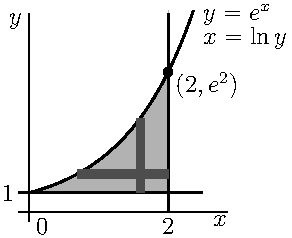
\includegraphics{domain4a.pdf}} \qquad
  (b) \raisebox{-0.5\height}{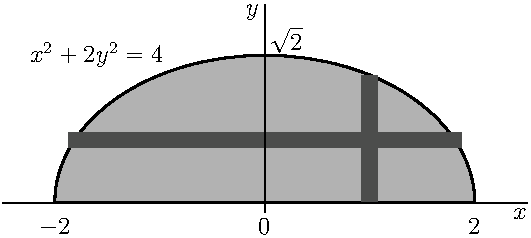
\includegraphics{domain4b.pdf}} 
\end{center}
\begin{center}
  (c) \raisebox{-0.5\height}{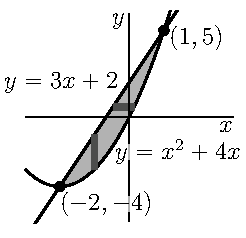
\includegraphics{domain4c.pdf}}     \end{center}

\leqnomode
\begin{align*}
\int_0^2 \dee{x}\int_1^{e^x} \dee{y}
&=\int_0^2 \dee{x}\ \big[e^x-1\big]
=\big[e^x-x\big]_0^2
=e^2-3
\tag{a} \\
\int_0^{e^2} \dee{y}\int_{\ln y}^2 \dee{x}
&=\int_0^{e^2} \dee{y}\ \big[2-\ln y\big]
=\big[2y-y\ln y+y\big]_1^{e^2}
=e^2-3\notag \displaybreak[0]\\
\noalign{\smallskip}
%%%
\int_0^{\sqrt{2}}\dee{y}\int_{-\sqrt{4-2y^2}}^{\sqrt{4-2y^2}}\dee{x}\ y
&=\int_0^{\sqrt{2}}\dee{y}\ 2y\sqrt{4-2y^2}
=-\frac{1}{3}\Big[{(4-2y^2)}^{3/2}\Big]_0^{\sqrt{2}}
=\frac{8}{3}
\tag{b} \\
\int_{-2}^{2} \dee{x}\int_0^{\sqrt{2-{x^2\over 2}}} \dee{y}\ y
&=\int_{-2}^{2} \dee{x}\ \left[1-\frac{x^2}{4}\right]
=2\int_0^{2} \dee{x}\ \left[1-\frac{x^2}{4}\right]
=2\left[x-\frac{x^3}{12}\right]_0^{2}
=\frac{8}{3}\notag\displaybreak[0]\\
\noalign{\smallskip}
%%%
\int_{-2}^1 \dee{x}\int_{x^2+4x}^{3x+2}\dee{y}
&=\int_{-2}^1 \dee{x}\ \big[-x^2-x+2\big]
=\left[-\frac{x^3}{3}-\frac{x^2}{2}+2x\right]_{-2}^1
=\frac{9}{2}
\tag{c} \\
\int_{-4}^{5} \dee{y}\int_{{y-2\over 3}}^{-2+\sqrt{4+y}} \dee{x}
&=\int_{-4}^{5} \dee{y}\ \left[\!-\frac{4}{3}-\frac{y}{3}+\sqrt{4+y}\right]
=\left[-\frac{4y}{3}-\frac{y^2}{6}+\frac{2}{3}{(4+y)}^{3\over 2}\right]_{-4}^{5}
\notag \\
&=\frac{9}{2}\notag
\end{align*}
In part (c), we used that the equation $y=x^2+4x$ is equivalent to 
$y+4=(x+2)^2$ and hence to $x=-2\pm\sqrt{y+4}$.
\reqnomode
\end{solution}

%%%%%%%%%%%%%%%%%%%%%%%%%%%%%%%%
\begin{question}[M200 2006A] %6
Combine the sum of the two iterated double integrals
\begin{equation*}
\int_{y=0}^{y=1}\int_{x=0}^{x=y} f(x,y)\ \dee{x}\,\dee{y}
+\int_{y=1}^{y=2}\int_{x=0}^{x=2-y} f(x,y)\ \dee{x}\,\dee{y}
\end{equation*}
into a single iterated double integral with the order of 
integration reversed.
\end{question}

%\begin{hint}
%
%\end{hint}

\begin{answer}
$\int_{x=0}^{x=1}\int_{y=x}^{y=2-x} f(x,y)\ \dee{y}\,\dee{x}$
\end{answer}

\begin{solution}
In the given integrals
\begin{itemize}
\item
$y$ runs for $0$ to $2$, and

\item
for each fixed $y$ between $0$ and $1$, $x$ runs from $0$ to $y$
and


\item
for each fixed $y$ between $1$ and $2$, $x$ runs from $0$ to $2-y$
\end{itemize}
The figure on the left below contains a sketch of that region together
with the generic horizontal slices that were used to set up the given
integrals.
\begin{center}
     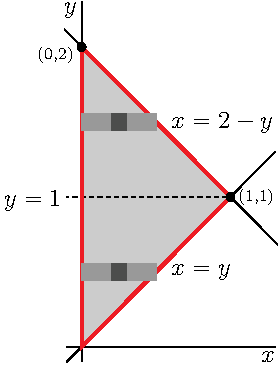
\includegraphics{OE06A_6h.pdf}\qquad
     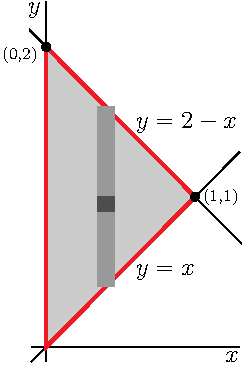
\includegraphics{OE06A_6v.pdf}
\end{center}
To reverse the order of integration, we switch to vertical, rather
than horizontal, slices, as in the figure on the right above.
Looking at that figure, we see that 
\begin{itemize}
\item
$x$ runs for $0$ to $1$, and

\item
for each fixed $x$ in that range, $y$ runs from $x$ to $2-x$.
\end{itemize}
So the desired integral is
\begin{align*}
\int_{x=0}^{x=1}\int_{y=x}^{y=2-x} f(x,y)\ \dee{y}\,\dee{x}
\end{align*}
\end{solution}

%%%%%%%%%%%%%%%%%%%%%%%%%%%%%%%%
\begin{question}[M200 2004A] %7
Consider the integral
\begin{equation*}
\int_0^1\int_x^1 e^{x/y}\ \dee{y}\ \dee{x}
\end{equation*}
\begin{enumerate}[(a)]
\item
Sketch the domain of integration.
\item
Evaluate the integral by reversing the order of integration.
\end{enumerate}
\end{question}

%\begin{hint}
%
%\end{hint}

\begin{answer}
(a)

\begin{center}
     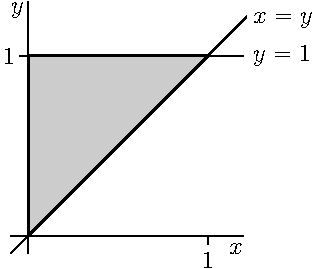
\includegraphics{OE04Q7a.pdf}
\end{center}

(b) $\half(e-1)$
\end{answer}

\begin{solution}
(a) In the given integral
\begin{itemize}
\item 
  $x$ runs from $0$ to $1$ and
\item
  for each fixed $x$ between $0$ and $1$, $y$ runs from $x$ to $1$ 
\end{itemize}
So the domain of integration is 
\begin{equation*}
D = \Set{(x,y)}{0\le x\le 1,\ x\le y\le 1}
\end{equation*}
It is sketched in the figure on the left below.

\begin{center}
     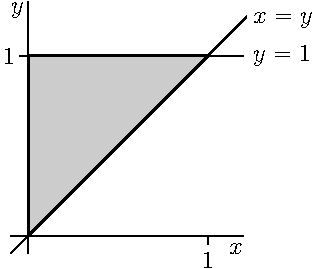
\includegraphics{OE04Q7a.pdf}\qquad
     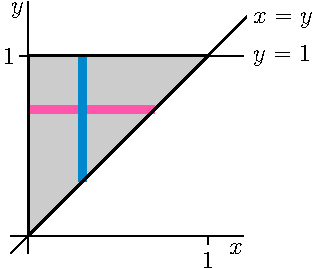
\includegraphics{OE04Q7.pdf}
\end{center}


(b) The given integral decomposed the domain of integration into 
vertical strips like the blue strip in the figure on the right above. 
To reverse the order of integration, we instead use horizontal strips. 
Looking at the pink strip in the figure on the right above, we see that 
this entails
\begin{itemize}
\item 
  having $y$ run from $0$ to $1$ and
\item
  for each fixed $y$ between $0$ and $1$, having $x$ run from $0$ to $y$ 
\end{itemize}
This gives
\begin{equation*}
\int_0^1\dee{y}\int_0^y \dee{x}\ e^{x/y}=\int_0^1\dee{y}\ \Big[ye^{x/y}\Big]_0^y
=\int_0^1\dee{y}\ y(e-1)
=\frac{1}{2} (e-1)
\end{equation*}
\end{solution}

%%%%%%%%%%%%%%%%%%%%%%%%%%%%%%%%
\begin{question}[M200 2006D] %4
The integral $I$ is defined as
\begin{equation*}
I =\dblInt_R f(x,y)\ \dee{A}
  = \int_1^{\sqrt{2}} \int_{1/y}^{\sqrt{y}} f(x,y)\,\dee{x}\,\dee{y}
    +\int_{\sqrt{2}}^4 \int_{y/2}^{\sqrt{y}} f(x,y)\,\dee{x}\,\dee{y}
\end{equation*}


\begin{enumerate}[(a)]
\item
 Sketch the region $R$.

\item
 Re--write the integral $I$ by reversing the order of integration.

\item Compute the integral $I$ when $f(x,y)= x/y$.
\end{enumerate}
\end{question}

%\begin{hint}
%
%\end{hint}

\begin{answer}
(a) The region $R$ is the shaded region in the figure

\begin{center}
     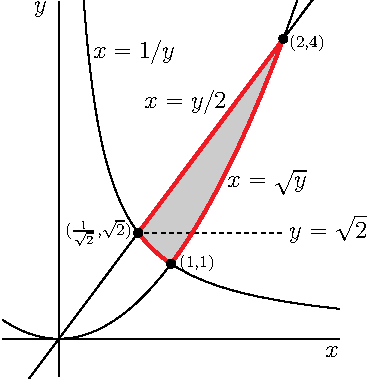
\includegraphics{OE06D_4.pdf}
\end{center}

(b) $I= \int_{1/\sqrt{2}}^1 \int_{1/x}^{2x} f(x,y)\,\dee{y}\,\dee{x}
    +\int_1^2 \int_{x^2}^{2x} f(x,y)\,\dee{y}\,\dee{x}$ \qquad
(c) $\frac{1}{2}$
\end{answer}

\begin{solution}
(a) On $R$
\begin{itemize}
\item
$y$ runs from $1$ to $4$ (from $1$ to $\sqrt{2}$ in the first integral and
from $\sqrt{2}$ to $4$ in the second).
\item 
For each fixed $y$ between $1$ and $\sqrt{2}$, $x$ runs from $\frac{1}{y}$
to $\sqrt{y}$ and 
\item 
for each fixed $y$ between $\sqrt{2}$ and $4$, $x$ runs from $\frac{y}{2}$
to $\sqrt{y}$.
\end{itemize}
The figure on the left below is a sketch of $R$, together with 
generic horizontal strips as were used in setting up the integral.

\begin{center}
     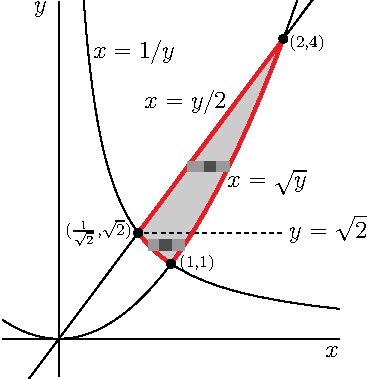
\includegraphics{OE06D_4h.pdf}\qquad
     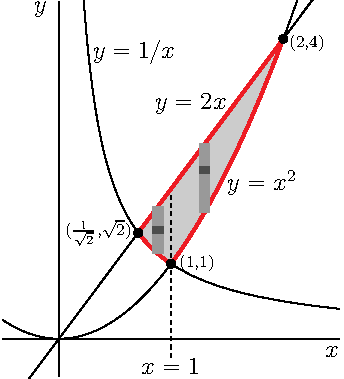
\includegraphics{OE06D_4v.pdf}
\end{center}

(b) To reverse the order of integration we use vertical strips as in
the figure on the right above. Looking at that figure, we see that, on $R$,
\begin{itemize}
\item
$x$ runs from $1/\sqrt{2}$ to $2$.
\item 
For each fixed $x$ between $1/\sqrt{2}$ and $1$, $y$ runs from $\frac{1}{x}$
to $2x$ and 
\item 
for each fixed $x$ between $1$ and $2$, $y$ runs from $x^2$
to $2x$.
\end{itemize}
So
\begin{align*}
I= \int_{1/\sqrt{2}}^1 \int_{1/x}^{2x} f(x,y)\,\dee{y}\,\dee{x}
    +\int_1^2 \int_{x^2}^{2x} f(x,y)\,\dee{y}\,\dee{x}
\end{align*}

(c) When $f(x,y)=\frac{x}{y}$,
\begin{align*}
I &= \int_1^{\sqrt{2}} \int_{1/y}^{\sqrt{y}} \frac{x}{y}\,\dee{x}\,\dee{y}
    +\int_{\sqrt{2}}^4 \int_{y/2}^{\sqrt{y}} \frac{x}{y}\,\dee{x}\,\dee{y} \\
  &=\int_1^{\sqrt{2}} \frac{1}{y}\left[\frac{y}{2}-\frac{1}{2y^2}\right]
                                               \,\dee{y}
    +\int_{\sqrt{2}}^4 \frac{1}{y}\left[\frac{y}{2}-\frac{y^2}{8}\right]
                                               \,\dee{y} \\
  &=\left[\frac{y}{2}+\frac{1}{4y^2}\right]_1^{\sqrt{2}}
    +\left[\frac{y}{2}-\frac{y^2}{16}\right]_{\sqrt{2}}^4 
   =\frac{1}{\sqrt{2}} +\frac{1}{8}-\frac{1}{2}-\frac{1}{4}
     +2 -1 -\frac{1}{\sqrt{2}} +\frac{1}{8} \\
  &=\frac{1}{2}
\end{align*}
\end{solution}

%%%%%%%%%%%%%%%%%%%%%%%%%%%%%%%%
\begin{question}[M200 2007A] \label{prob_s3.1f}  %7
A region $E$ in the $xy$--plane has the property that for all 
continuous functions f
\begin{equation*}
\dblInt_E f(x,y)\,\dee{A}
= \int_{x=-1}^{x=3}\left[\int_{y=x^2}^{y=2x+3} f(x,y) \dee{y}\right] \dee{x}
\end{equation*}

\begin{enumerate}[(a)]
\item 
 Compute $\dblInt_E x\,\dee{A}$.
 
\item 
 Sketch the region E.

\item
 Set up $\dblInt_E x\,\dee{A}$ as an integral or sum of integrals 
in the opposite order.
\end{enumerate}
\end{question}

%\begin{hint}
%
%\end{hint}

\begin{answer}
(a) $\frac{32}{3}$

(b)

\begin{center}
     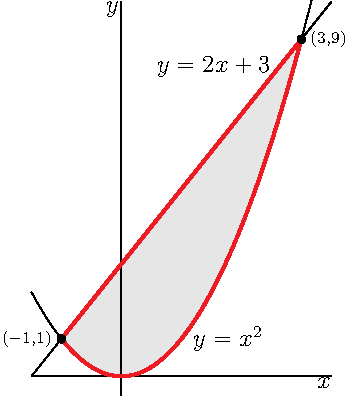
\includegraphics[scale=0.75]{OE07A_7.pdf}
\end{center}

(c) $I = \int_0^1\dee{y} \int_{-\sqrt{y}}^{\sqrt{y}}\dee{x}\ x
    +\int_1^9\dee{y} \int_{(y-3)/2}^{\sqrt{y}}\dee{x}\ x$
\end{answer}

\begin{solution}
(a) When $f(x,y)=x$,
\begin{align*}
\int_{x=-1}^{x=3}\left[\int_{y=x^2}^{y=2x+3} x \dee{y}\right] \dee{x}
&= \int_{x=-1}^{x=3}\left[x(2x+3-x^2) \right] \dee{x} \\
&=\left[\frac{2x^3}{3}+\frac{3x^2}{2}-\frac{x^4}{4}\right]_{-1}^3
=18+\frac{27}{2}-\frac{81}{4} +\frac{2}{3}-\frac{3}{2}+\frac{1}{4} \\
&=18+12-20+\frac{2}{3}
=\frac{32}{3}
\end{align*}

(b) On the region $E$
\begin{itemize}
\item
 $x$ runs from $-1$ to $3$ and
\item
 for each $x$ in that range, $y$ runs from $x^2$ to $2x+3$
\end{itemize}
Here are two sketches of $E$, with the left one including a generic 
vertical strip as was used in setting up the given integral.
\begin{center}
     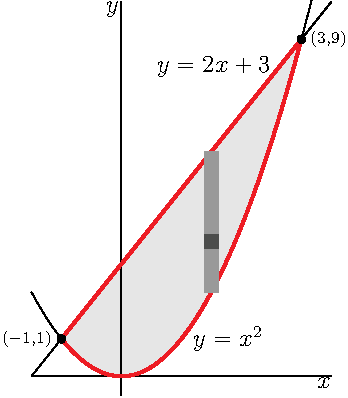
\includegraphics{OE07A_7v.pdf}\qquad
     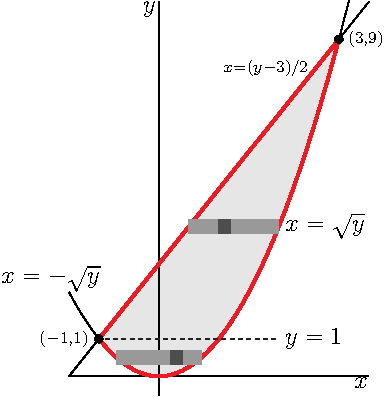
\includegraphics{OE07A_7h.pdf}
\end{center}

(c) To reverse the order of integration we use horizontal strips
as in the figure on the right above. Looking at that figure, we see that,
on the region $E$,
\begin{itemize}
\item
 $y$ runs from $0$ to $9$ and
\item
 for each $y$ between $0$ and $1$, $x$ runs from $-\sqrt{y}$ to $\sqrt{y}$
\item
 for each $y$ between $1$ and $9$, $x$ runs from $(y-3)/2$ to $\sqrt{y}$
\end{itemize}
So
\begin{align*}
I = \int_0^1\dee{y} \int_{-\sqrt{y}}^{\sqrt{y}}\dee{x}\ x
    +\int_1^9\dee{y} \int_{(y-3)/2}^{\sqrt{y}}\dee{x}\ x
\end{align*}
\end{solution}

%%%%%%%%%%%%%%%%%%%%%%%%%%%%%%%%
\begin{question}[M200 2008A] %2
Calculate the integral:
\begin{equation*}
\dblInt_D \sin(y^2)\ \dee{A}
\end{equation*}
where $D$ is the region bounded by $x + y = 0$, $2x - y = 0$, and $y = 4$.
\end{question}

\begin{hint}
The antiderivative of the function $\sin(y^2)$ cannot be expressed
in terms of familiar functions. So we do not want the inside integral to 
be over $y$.
\end{hint}

\begin{answer}
$\frac{3}{4}\big[1-\cos(16)\big]$
\end{answer}

\begin{solution}
The antiderivative of the function $\sin(y^2)$ cannot be expressed
in terms of familiar functions. So we do not want the inside integral to 
be over $y$. So we'll use horizontal slices as in the figure

\begin{center}
     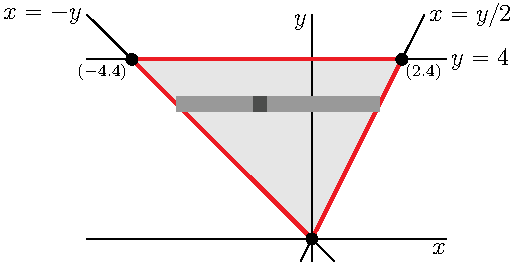
\includegraphics{OE08A_2.pdf}
\end{center}
  
On the domain of integration
\begin{itemize}
\item
   $y$ runs from $0$ to $4$, and
\item
   for each fixed $y$ in that range, $x$ runs from $-y$ to $y/2$
\end{itemize}
The given integral
\begin{align*}
\dblInt_D \sin(y^2)\ \dee{A}
&=\int_0^4\dee{y}\int_{-y}^{y/2}\dee{x}\ \sin(y^2) \\
&=\int_0^4 \dee{y}\ \frac{3}{2}y\,\sin(y^2) \\
&=\left[-\frac{3}{4}\cos(y^2)\right]_0^4 \\
&=\frac{3}{4}\big[1-\cos(16)\big]
\end{align*}

\end{solution}

%%%%%%%%%%%%%%%%%%%%%%%%%%%%%%%%
\begin{question}[M200 2008D] %6
Consider the integral
\begin{equation*}
I = \int_0^1 \int_{\sqrt{y}}^1 \frac{\sin(\pi x^2)}{x}\ \dee{x}\,\dee{y}
\end{equation*}

\begin{enumerate}[(a)]
\item
Sketch the region of integration.
\item 
Evaluate I.

\end{enumerate}
\end{question}

\begin{hint}
The inside integral, $\int_{\sqrt{y}}^1 \frac{\sin(\pi x^2)}{x}\ \dee{x}$,
in the given form of $I$ looks really nasty.  So try exchanging
the order of integration.
\end{hint}

\begin{answer}
(a)
\begin{center}
     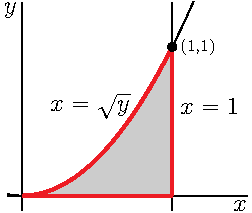
\includegraphics{OE08D_6.pdf}
\end{center}

(b) $\frac{1}{\pi}$
\end{answer}

\begin{solution}
(a)
On the domain of integration
\begin{itemize}
\item
$y$ runs from $0$ to $1$ and
\item
for each fixed $y$ in that range, $x$ runs from $\sqrt{y}$
to $1$.
\end{itemize}
The figure on the left below is a sketch of that domain, together with 
a generic horizontal strip as was used in setting up the integral.

\begin{center}
     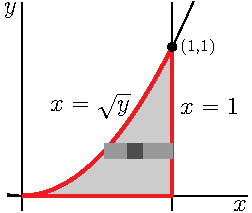
\includegraphics{OE08D_6h.pdf}\qquad
     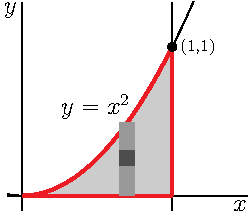
\includegraphics{OE08D_6v.pdf}\qquad
\end{center}

(b) The inside integral, $\int_{\sqrt{y}}^1 \frac{\sin(\pi x^2)}{x}\ \dee{x}$,
in the given form of $I$ looks really nasty.  So let's try exchanging
the order of integration. Looking at the figure on the right above,
we see that, on  the domain of integration,
\begin{itemize}
\item
$x$ runs from $0$ to $1$ and
\item
for each fixed $x$ in that range, $y$ runs from $0$
to $x^2$.
\end{itemize}
So
\begin{align*}
I &= \int_0^1\dee{x}\int_0^{x^2}\dee{y}\ \frac{\sin(\pi x^2)}{x} \\
  &=\int_0^1\dee{x}\ x\sin(\pi x^2) \\
  &=\left[-\frac{\cos(\pi x^2)}{2 \pi}\right]_0^1 
             \qquad\text{(Looks pretty rigged!)}\\
  &=\frac{1}{\pi}
\end{align*}
\end{solution}

%%%%%%%%%%%%%%%%%%%%%%%%%%%%%%%%
\begin{question}[M200 2009A] %1
Let $I$ be the double integral of the function $f(x,y) = y^2 \sin xy$ 
over the triangle with vertices $(0, 0)$, $(0, 1)$ and $(1, 1)$ 
in the $xy$--plane.

\begin{enumerate}[(a)]
\item
Write $I$ as an iterated integral in two different ways.

\item 
Evaluate $I$.

\end{enumerate}
\end{question}

%\begin{hint}
%
%\end{hint}

\begin{answer}
(a) $I=\int_0^1\dee{x}\int_x^1\dee{y}\ y^2\sin xy  
           =\int_0^1\dee{y}\int_0^y\dee{x}\ y^2\sin xy$

(b) $\frac{1-\sin 1}{2}$
\end{answer}

\begin{solution}
(a) Let's call the triangle $\cT$.
Here are two sketches of $\cT$, one including a generic vertical strip
and one including a generic horizontal strip. Notice that the equation
of the line through $(0,0)$ and $(1,1)$ is $y=x$.

\begin{center}
     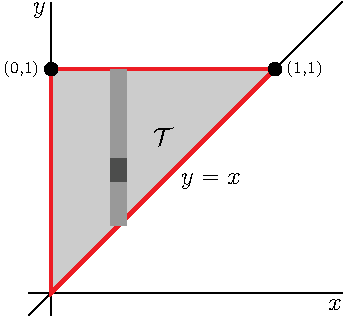
\includegraphics{OE09A_5v.pdf}\qquad
     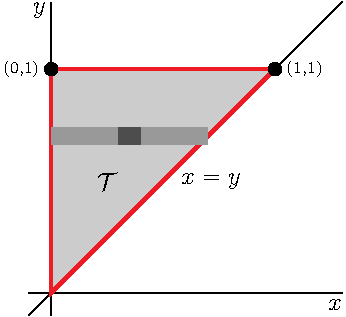
\includegraphics{OE09A_5h.pdf}\qquad
\end{center}

First, we'll set up the integral using vertical strips. Looking
at the figure on the left above, we see that, on $\cT$,
\begin{itemize}
\item
$x$ runs from $0$ to $1$ and
\item
for each $x$ in that range, $y$ runs from $x$ to $1$.
\end{itemize}
So the integral
\begin{align*}
I=\int_0^1\dee{x}\int_x^1\dee{y}\ y^2\sin xy
\end{align*}

Next, we'll set up the integral using horizontal strips. Looking
at the figure on the right above, we see that, on $\cT$,
\begin{itemize}
\item
$y$ runs from $0$ to $1$ and
\item
for each $y$ in that range, $x$ runs from $0$ to $y$.
\end{itemize}
So the integral
\begin{align*}
I=\int_0^1\dee{y}\int_0^y\dee{x}\ y^2\sin xy
\end{align*}

(b) To evaluate the inside integral,  $\int_x^1\dee{y}\ y^2\sin xy$,
of the vertical strip version, will require two integration by
parts to get rid of the $y^2$. So we'll use the horizontal strip version.
\begin{align*}
I&=\int_0^1\dee{y}\int_0^y\dee{x}\ y^2\sin xy \\
&=\int_0^1\dee{y}\ \Big[-y\cos xy\Big]_0^y \\
&=\int_0^1\dee{y}\ \big[y-y\cos y^2\big] \\
&=\left[\frac{y^2}{2}-\frac{\sin y^2}{2}\right]_0^1
\qquad\text{(Look's pretty rigged!)} \\
&= \frac{1-\sin 1}{2}
\end{align*}

\end{solution}

%%%%%%%%%%%%%%%%%%%%%%%%%%%%%%%%
\begin{question}[M200 2009D] %5
Find the volume $(V)$ of the solid bounded above by the surface
\begin{equation*}
z = f (x,y) = e^{-x^2},
\end{equation*}
below by the plane $z = 0$ and over the triangle in the $xy$--plane
formed by the lines $x = 1$, $y = 0$ and $y = x$.

\end{question}

%\begin{hint}
%
%\end{hint}

\begin{answer}
$\frac{1-e^{-1}}{2}$
\end{answer}

\begin{solution}
If we call the triangular base region $\cT$, then the volume is
\begin{align*}
V=\dblInt_\cT f(x,y)\ \dee{A} = \dblInt_\cT e^{-x^2}\ \dee{x}\,\dee{y}
\end{align*}
If we set up the integral using horizontal slices, so that the inside integral
is the $x$--integral, there will be a big problem --- the integrand 
$e^{-x^2}$ does not have an obvious anti--derivative. (In fact its
antiderivative cannot be expressed in terms of familiar functions.)
So let's try vertical slices as in the sketch 
\begin{center}
      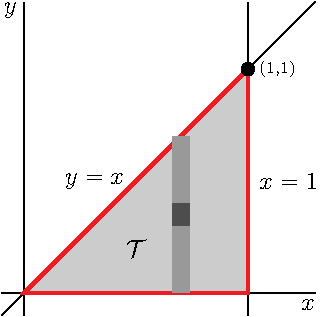
\includegraphics{OE09D_5.pdf}
\end{center}
Looking at that sketch we see that
\begin{itemize}
\item
$x$ runs from $0$ to $1$, and 
\item
for each $x$ in that range, $y$ runs from $0$ to $x$.
\end{itemize}
So the integral is
\begin{align*}
V&=\int_0^1\dee{x}\int_0^x\dee{y}\ e^{-x^2} \\
&=\int_0^1 \dee{x}\ xe^{-x^2} \\
&=\left[-\frac{1}{2}e^{-x^2}\right]_0^1 \\
&=\frac{1-e^{-1}}{2}
\end{align*}

\end{solution}

%%%%%%%%%%%%%%%%%%%%%%%%%%%%%%%%
\begin{question}[M200 2009D] %6
Consider the integral 
   $\displaystyle I=\int_0^1 \int_y^{2-y}\frac{y}{x} \ \dee{x}\,\dee{y}$.

\begin{enumerate}[(a)]
\item
Sketch the region of integration.

\item 
Interchange the order of integration.

\item
Evaluate $I$.
\end{enumerate}
\end{question}

%\begin{hint}
%
%\end{hint}

\begin{answer}
(a)
\begin{center}
     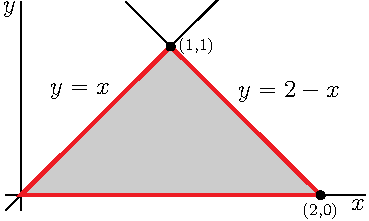
\includegraphics{OE09D_6.pdf}
\end{center}

(b) $I=\int_0^1\dee{x}\int_0^x\dee{y}\ \frac{y}{x}
  +\int_1^2\dee{x}\int_0^{2-x}\dee{y}\ \frac{y}{x}$\qquad
(c) $2\ln 2 -1$
\end{answer}

\begin{solution}
(a) On the domain of integration
\begin{itemize}
\item
$y$ runs from $0$ to $1$ and
\item
for each $y$ in that range $x$ runs from $y$ to $2-y$.
So the left hand side of the domain is the line $x=y$ and 
the right hand side of the domain is $x=2-y$.
\end{itemize}
The figure on the left below is a sketch of that domain, together with 
a generic horizontal strip as was used in setting up the integral.

\begin{center}
     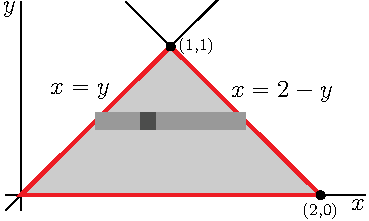
\includegraphics{OE09D_6h.pdf}\qquad
     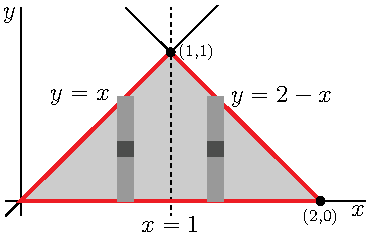
\includegraphics{OE09D_6v.pdf}\qquad
\end{center}

(b) 
To reverse the order of integration we use vertical, rather than horizontal, strips. Looking at the figure on the right above, we see that, in the
domain of integration
\begin{itemize}
\item
$x$ runs from $0$ to $2$ and
\item
for each $x$ between $0$ and $1$, $y$ runs from $0$ to $x$, while
\item
for each $x$ between $1$ and $2$, $y$ runs from $0$ to $2-x$.
\end{itemize}
So the integral
\begin{align*}
I=\int_0^1\dee{x}\int_0^x\dee{y}\ \frac{y}{x}
  +\int_1^2\dee{x}\int_0^{2-x}\dee{y}\ \frac{y}{x} 
\end{align*}

(c) Using the answer to part (b)
\begin{align*}
I&=\int_0^1\dee{x}\int_0^x\dee{y}\ \frac{y}{x}
  +\int_1^2\dee{x}\int_0^{2-x}\dee{y}\ \frac{y}{x} \\
&=\frac{1}{2}\int_0^1\dee{x}\ x
    +\frac{1}{2}\int_1^2\dee{x}\ \frac{(2-x)^2}{x}\\
&=\frac{1}{4} +\frac{1}{2}\int_1^2\dee{x}\ \left(\frac{4}{x}-4+x\right) \\
&=\frac{1}{4} +\frac{1}{2}\left[4\ln 2 -4 + \frac{4-1}{2}\right] \\
&=2\ln 2 -1
\end{align*}
\end{solution}

%%%%%%%%%%%%%%%%%%%%%%%%%%%%%%%%
\begin{question}[M200 2010A] %6
For the integral
\begin{equation*}
I = \int_0^1 \int_{\sqrt{x}}^1 \sqrt{1+y^3}\ \dee{y}\,\dee{x}
\end{equation*}
\begin{enumerate}[(a)]
\item
Sketch the region of integration.
\item
Evaluate $I$.
\end{enumerate}
\end{question}

\begin{hint}
The inside integral, $\int_{\sqrt{x}}^1 \sqrt{1+y^3}\ \dee{y}$,
of the given integral looks pretty nasty. Try reversing the order of 
integration.
\end{hint}

\begin{answer}
(a)
\begin{center}
     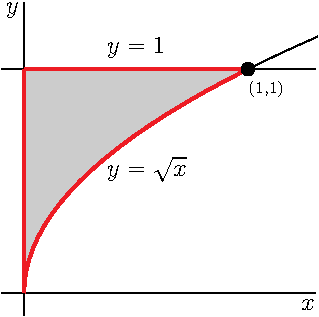
\includegraphics{OE10A_6.pdf}
\end{center}

(b) $\frac{2\big(2\sqrt{2}-1\big)}{9}$
\end{answer}

\begin{solution}
(a)
On the domain of integration,
\begin{itemize}
\item
$x$ runs from $0$ to $1$, and
\item
for each fixed $x$ in that range,
$y$ runs from $\sqrt{x}$ to $1$.
We may rewrite $y=\sqrt{x}$ as $x=y^2$, which is a rightward opening
parabola.
\end{itemize}
Here are two sketches of the domain of integration, which we call $D$.
The left hand sketch also shows a vertical slice, as was used in setting up 
the integral.
\begin{center}
     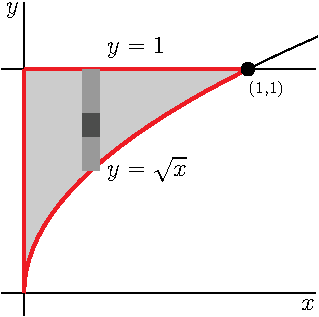
\includegraphics{OE10A_6v.pdf}\qquad
     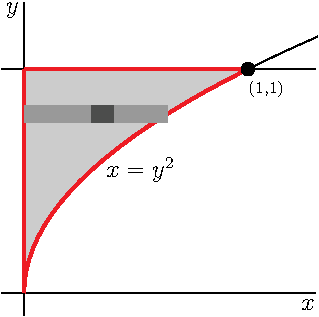
\includegraphics{OE10A_6h.pdf}
\end{center}

(b) The inside integral, $\int_{\sqrt{x}}^1 \sqrt{1+y^3}\ \dee{y}$,
of the given integral looks pretty nasty. So let's reverse the order of 
integration, by using horizontal, rather than vertical, slices.
Looking at the figure on the right above, we see that
\begin{itemize}
\item
$y$ runs from $0$ to $1$, and
\item
for each fixed $y$ in that range
$x$ runs from $0$ to $y^2$.
\end{itemize}
So
\begin{align*}
I &= \int_0^1\dee{y} \int_0^{y^2}\dee{x}\ \sqrt{1+y^3} \\
&=\int_0^1\dee{y} \ y^2\sqrt{1+y^3} \\
&=\int_1^2\frac{\dee{u}}{3}\ \sqrt{u}
\qquad\text{with $u=1+y^3,\ \dee{u}=3y^2\,\dee{y}$. Looks pretty rigged!} \\
&=\frac{1}{3} \left[\frac{u^{3/2}}{3/2}\right]_1^2 \\[0.05in]
&=\frac{2\big(2\sqrt{2}-1\big)}{9}
\end{align*}
\end{solution}

%%%%%%%%%%%%%%%%%%%%%%%%%%%%%%%%
\begin{question}[M200 2010D] %5
\begin{enumerate}[(a)]
\item
$D$ is the region bounded by the parabola $y^2 = x$ and the line $y = x - 2$.
Sketch $D$ and evaluate $J$ where
\begin{equation*}
J = \dblInt_D 3y\ \dee{A}
\end{equation*}
\item
Sketch the region of integration and then evaluate the integral $I$ :
\begin{equation*}
I = \int_0^4  \int_{\frac{1}{2}\sqrt{x}}^1  e^{y^3}\ \dee{y}\,\dee{x}
\end{equation*}
\end{enumerate}
\end{question}

\begin{hint}
(b) The inside integral, $\int_{\frac{1}{2}\sqrt{x}}^1  e^{y^3}\ \dee{y}$, 
looks pretty nasty because $e^{y^3}$ does not have an obvious antiderivative. 
Try reversing the order of integration. 
\end{hint}

\begin{answer}
(a) $J=\frac{27}{4}$

\begin{center}
     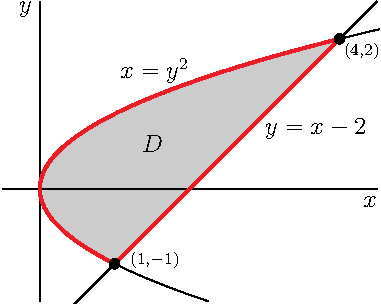
\includegraphics[scale=0.95]{OE10D_5a.pdf}
\end{center}


(b) $I=\frac{4}{3}\big[e-1\big]$

\begin{center}
     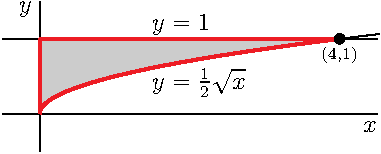
\includegraphics[scale=0.95]{OE10D_5b.pdf}
\end{center}
\end{answer}

\begin{solution}
(a) Observe that the parabola $y^2=x$ and the line $y=x-2$ meet
when $x=y+2$ and
\begin{equation*}
y^2=y+2
\iff y^2-y-2=0
\iff (y-2)(y+1)=0
\end{equation*}
So the points of intersection of $x=y^2$ and $y=x-2$ are $(1,-1)$
and $(4,2)$. Here is a sketch of $D$.

\begin{center}
     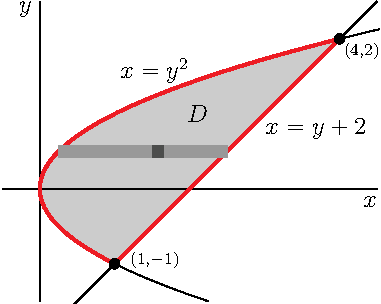
\includegraphics{OE10D_5aa.pdf}
\end{center}

To evaluate $J$, we'll use horizontal slices as in the figure above.
(If we were to use vertical slices we would have to split the integral in two,
with $0\le x\le 1$ in one part and $1\le x\le 4$ in the other.)
From the figure, we see that, on $D$,
\begin{itemize}
\item
$y$ runs from $-1$ to $2$ and
\item 
for each fixed $y$ in that range, $x$ runs from $y^2$ to $y+2$.
\end{itemize}
Hence
\begin{align*}
J &=\dblInt_D 3y\ \dee{A}
  =\int_{-1}^2\dee{y}\int_{y^2}^{y+2}\dee{x}\ 3y \\
  &=3\int_{-1}^2\dee{y}\ y(y+2-y^2) \\
  &=3\left[\frac{y^3}{3}+y^2-\frac{y^4}{4}\right]_{-1}^2 \\
  &=3\left[\frac{8}{3}+4-4+\frac{1}{3}-1+\frac{1}{4}\right] \\
  &=\frac{27}{4}
\end{align*}

(b) 
On the domain of integration,
\begin{itemize}
\item
$x$ runs from $0$ to $4$ and
\item 
for each fixed $x$ in that range, $y$ runs from $\frac{1}{2}\sqrt{x}$ to $1$.
\end{itemize}
The figure on the left below is a sketch of that domain, together with 
a generic vertical strip as was used in setting up the integral.

\begin{center}
     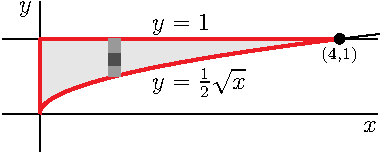
\includegraphics{OE10D_5bv.pdf}\qquad
     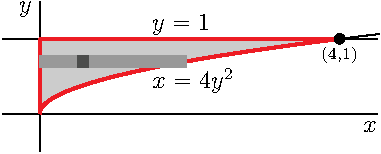
\includegraphics{OE10D_5bh.pdf}\qquad
\end{center}

The inside integral, over $y$, looks pretty nasty because $e^{y^3}$
does not have an obvious antiderivative. So let's reverse the order
of integration. That is, let's use horizontal, rather than vertical,
strips. From the figure on the right above, we see that, on the
domain of integration
\begin{itemize}
\item
$y$ runs from $0$ to $1$ and
\item 
for each fixed $y$ in that range, $x$ runs from $0$ to $4y^2$.
\end{itemize}
So 
\begin{align*}
I &= \int_0^1\dee{y}\int_0^{4y^2}\dee{x}\ e^{y^3} \\
  &= \int_0^1\dee{y}\ 4y^2 e^{y^3} \\
  &= \frac{4}{3}\int_0^1\dee{u}\ e^u \qquad\text{with }
                 u=y^3,\ \dee{u}=3y^2\,\dee{y}\qquad
                 \text{(Looks rigged!)}\\
  &=\frac{4}{3}\big[e-1\big]
\end{align*}
\end{solution}

%%%%%%%%%%%%%%%%%%%%%%%%%%%%%%%%
\begin{question}[M200 2011D] %5a
Consider the iterated integral
\begin{equation*}
\int_{-4}^0\int_{\sqrt{-y}}^2 \cos(x^3)\,\dee{x}\,\dee{y}
\end{equation*}
\begin{enumerate}[(a)]
\item
Draw the region of integration.
\item
Evaluate the integral.
\end{enumerate}
\end{question}

\begin{hint}
(b) The inside integral, $\int_{\sqrt{-y}}^2 \cos(x^3)\,\dee{x}$
looks nasty. Try reversing the order of integration.
\end{hint}

\begin{answer}
(a) 

\begin{center}
     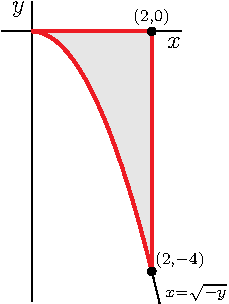
\includegraphics{OE11D_5.pdf}
\end{center}

(b) $\frac{\sin(8)}{3}$
\end{answer}

\begin{solution}
(a)  On the domain of integration
\begin{itemize}
\item 
  $y$ runs from $-4$ to $0$ and
\item
  for each $y$ in that range, $x$ runs from $\sqrt{-y}$ (when $y=-x^2$)
  to $2$.
\end{itemize}
The figure on the left below provides a sketch of the domain of integration.
It also shows the generic horizontal slice that was used to set up the given 
iterated integral.

\begin{center}
     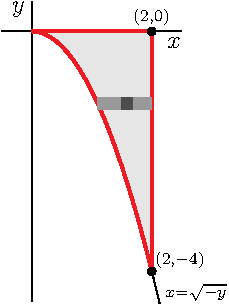
\includegraphics{OE11D_5a.pdf}\qquad
     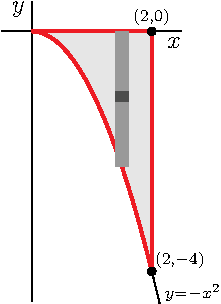
\includegraphics{OE11D_5b.pdf}
\end{center}


(b) The inside integral, $\int_{\sqrt{-y}}^2 \cos(x^3)\,\dee{x}$
looks nasty. So let's reverse the order of integration and use vertical,
rather than horizontal, slices. From the
figure on the right above, on the domain of integration,
\begin{itemize}
\item 
  $x$ runs from $0$ to $2$ and
\item
  for each $x$ in that range, $y$ runs from $-x^2$ 
  to $0$.
\end{itemize}
So the integral
\begin{align*}
\int_{-4}^0\int_{\sqrt{-y}}^2 \cos(x^3)\,\dee{x}\,\dee{y}
&=\int_0^2\dee{x}\int_{-x^2}^0\dee{y}\ \cos(x^3) \\
&=\int_0^2\dee{x}\ x^2\ \cos(x^3) 
=\left[\frac{\sin(x^3)}{3}\right]_0^2 \\
&=\frac{\sin(8)}{3}
\end{align*}
\end{solution}


%%%%%%%%%%%%%%%%%%%%%%%%%%%%%%%%
\begin{question}[M200 2012A] %6
\begin{enumerate}[(a)]
\item
Combine the sum of the iterated integrals
\begin{equation*}
I = \int_0^1\int_{-\sqrt{y}}^{\sqrt{y}} f(x,y)\ \dee{x}\,\dee{y}
   + \int_1^4\int_{y-2}^{\sqrt{y}} f(x,y)\ \dee{x}\,\dee{y}
\end{equation*}
into a single iterated integral with the order of integration reversed.
\item
Evaluate $I$ if $f(x,y)=\frac{e^x}{2-x}$.
\end{enumerate}
\end{question}

%\begin{hint}
%
%\end{hint}

\begin{answer}
(a) $I = \int_{-1}^2\int_{x^2}^{x+2} f(x,y)\ \dee{y}\,\dee{x}$\qquad
(b) $ 2e^2 + \frac{1}{e}$
\end{answer}

\begin{solution}
(a)  On the domain of integration
\begin{itemize}
\item 
  $y$ runs from $0$ to $4$ and
\item
  for each $y$ in the range $0\le y\le 1$, $x$ runs from $-\sqrt{y}$ 
to $\sqrt{y}$ and
\item
  for each $y$ in the range $1\le y\le 4$, $x$ runs from $y-2$ 
to $\sqrt{y}$.
\end{itemize}
Both figures below provide sketches of the domain of integration.

\begin{center}
     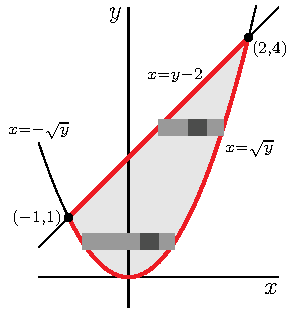
\includegraphics{OE12A_6a.pdf}\qquad
     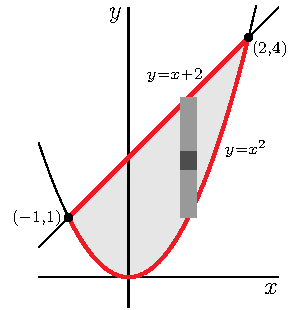
\includegraphics{OE12A_6b.pdf}
\end{center}

To reverse the order of integration observe, from the figure on the
right above that, on the domain of integration,
\begin{itemize}
\item 
  $x$ runs from $-1$ to $2$ and
\item
  for each $x$ in that range, $y$ runs from $x^2$ 
  to $x+2$.
\end{itemize}
So the integral
\begin{equation*}
I = \int_{-1}^2\int_{x^2}^{x+2} f(x,y)\ \dee{y}\,\dee{x}
\end{equation*}

(b) We'll use the integral with the order of integration reversed
that we found in part (a). When $f(x,y)=\frac{e^x}{2-x}$
\begin{align*}
I &= \int_{-1}^2\int_{x^2}^{x+2} \frac{e^x}{2-x}\ \dee{y}\,\dee{x} \\
  &= \int_{-1}^2 (x+2-x^2)\frac{e^x}{2-x}\ \dee{x} 
   = -\int_{-1}^2 (x-2)(x+1)\frac{e^x}{2-x}\ \dee{x} \\
  &= \int_{-1}^2 (x+1) e^x\ \dee{x} \\
  &= \Big[xe^x\Big]_{-1}^2 \\
  &= 2e^2 + \frac{1}{e}
\end{align*}
\end{solution}

%%%%%%%%%%%%%%%%%%%%%%%%%%%%%%%%
\begin{question}[M200 2012D] %7
Let
\begin{equation*}
I=\int_0^4\int_{\sqrt{y}}^{\sqrt{8-y}} f(x,y)\,\dee{x}\,\dee{y}
\end{equation*}
\begin{enumerate}[(a)]
\item
Sketch the domain of integration.
\item
Reverse the order of integration.
\item
Evaluate the integral for $f(x,y)=\frac{1}{(1+y)^2}$.
\end{enumerate}
 
\end{question}

\begin{hint}
 $\frac{1}{9-x^2} =\frac{1}{6}\left(\frac{1}{x+3}-\frac{1}{x-3}\right)$.
\end{hint}

\begin{answer}
(a)
\begin{center}
     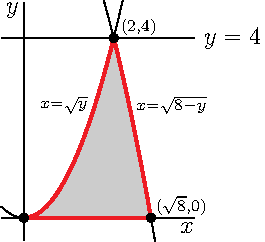
\includegraphics{OE12D_7aa.pdf}
\end{center}

(b) $\int_0^2\int_0^{x^2} f(x,y)\,\dee{y}\,\dee{x}
+\int_2^{\sqrt{8}}\int_0^{8-x^2} f(x,y)\,\dee{y}\,\dee{x}$\qquad
(c) $\sqrt{8}-\arctan 2 -\frac{1}{6}\left[\ln\frac{3+\sqrt{8}}{3-\sqrt{8}}
                                       -\ln 5\right]$
\end{answer}

\begin{solution}
On the domain of integration 
\begin{itemize}
\item
$y$ runs from $0$ to $4$. In inequalities, $0\le y\le 4$.
\item
For each fixed $y$ in that range, $x$ runs from $\sqrt{y}$ to
$\sqrt{8-y}$. In inequalities, that is $\sqrt{y}\le x\le \sqrt{8-y}$,
or $y\le x^2\le 8-y$.
\end{itemize}
Here are two sketchs of the domain of integration.

\begin{center}
     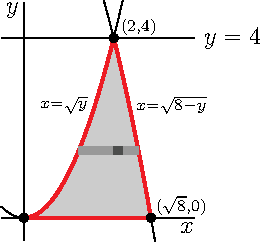
\includegraphics{OE12D_7a.pdf}\qquad\qquad
     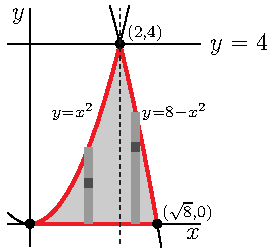
\includegraphics{OE12D_7b.pdf}
\end{center}


(b) To reverse the order we observe, from the figure on the right above,
that, on the domain of integration,
\begin{itemize}
\item
$x$ runs from $0$ to $\sqrt{8}$. In inequalities, $0\le x\le \sqrt{8}$.
\item
For each fixed $x$ between $0$ and $2$, $y$ runs from $0$ to
$x^2$. In inequalities, that is $0\le y\le x^2$.
\item
For each fixed $x$ between $2$ and $\sqrt{8}$, $y$ runs from $0$ to
$8-x^2$. In inequalities, that is $0\le y\le 8-x^2$.
\end{itemize}
So the integral is
\begin{equation*}
\int_0^2\int_0^{x^2} f(x,y)\,\dee{y}\,\dee{x}
+\int_2^{\sqrt{8}}\int_0^{8-x^2} f(x,y)\,\dee{y}\,\dee{x}
\end{equation*}

(c) We'll use the form of part (b).
\begin{align*}
&\int_0^2\int_0^{x^2} \frac{1}{(1+y)^2}\,\dee{y}\,\dee{x}
+\int_2^{\sqrt{8}}\int_0^{8-x^2} \frac{1}{(1+y)^2}\,\dee{y}\,\dee{x} \\
&=-\int_0^2 \left[\frac{1}{1+y}\right]_0^{x^2}\,\dee{x}
-\int_2^{\sqrt{8}} \left[\frac{1}{1+y}\right]_0^{8-x^2}\,\dee{x} \\
&=\int_0^2 \left[1-\frac{1}{1+x^2}\right]\,\dee{x}
+\int_2^{\sqrt{8}} \left[1-\frac{1}{9-x^2}\right]\,\dee{x} \\
&=\sqrt{8}-\arctan x\bigg|_0^2
  -\frac{1}{6}\int_2^{\sqrt{8}} 
         \left[\frac{1}{3+x}+\frac{1}{3-x}\right]\,\dee{x} \\
&=\sqrt{8}-\arctan 2 -\frac{1}{6}\Big[\ln(3+x)-\ln(3-x)\Big]_2^{\sqrt{8}} \\
&=\sqrt{8}-\arctan 2 -\frac{1}{6}\left[\ln\frac{3+\sqrt{8}}{3-\sqrt{8}}
                                       -\ln 5\right] 
\end{align*}
\end{solution}

\begin{question}[M200 2013D] %6
Evaluate
\begin{equation*}
\int_{-1}^0 \int_{-2}^{2x} e^{y^2}\ \dee{y}\,\dee{x}
\end{equation*}
\end{question}

\begin{hint}
The antiderivative of the function $e^{-y^2}$ cannot be expressed
in terms of elementary functions. So the inside integral 
$\int_{-2}^{2x} e^{y^2}\ \dee{y}$ cannot be evaluated using 
standard calculus 2 techniques. Try reversing the order of integration.
\end{hint}

\begin{answer}
$\frac{1}{4}\big[e^4-1\big]$
\end{answer}

\begin{solution}
The antiderivative of the function $e^{-y^2}$ cannot be expressed
in terms of elementary functions. So the inside integral 
$\int_{-2}^{2x} e^{y^2}\ \dee{y}$ cannot be evaluated using 
standard calculus 2 techniques. The trick for dealing with this
integral is to reverse the order of integration.
On the domain of integration 
\begin{itemize}
\item
$x$ runs from $-1$ to $0$. In inequalities, $-1\le x\le 0$.
\item
For each fixed $x$ in that range, $y$ runs from $-2$ to
$2x$. In inequalities,  $-2\le y\le 2x$.
\end{itemize}
The domain of integration, namely
\begin{equation*}
\Set{(x,y)}{-1\le x\le 0,\ -2\le y\le 2x}
\end{equation*} 
is sketched in the figure on the left below.

\begin{center}
     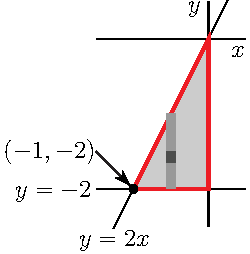
\includegraphics{OE13D_6a.pdf}\qquad
     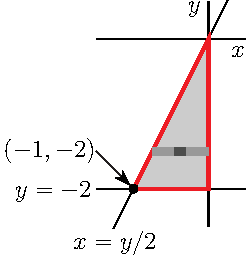
\includegraphics{OE13D_6b.pdf}
\end{center}

Looking at the figure on the right above, we see that we can also 
express the domain of integration as
\begin{equation*}
\Set{(x,y)}{-2\le y\le 0,\ y/2\le x\le 0}
\end{equation*} 
So the integral 
\begin{align*}
\int_{-1}^0 \int_{-2}^{2x} e^{y^2}\ \dee{y}\,\dee{x}
&=\int_{-2}^0 \int_{y/2}^{0} e^{y^2}\ \dee{x}\,\dee{y} \\
&=-\frac{1}{2}\int_{-2}^0  y e^{y^2}\ \dee{y} \\
&=-\frac{1}{2}\left[\frac{1}{2}e^{y^2}\right]_{-2}^0 \\
&=\frac{1}{4}\big[e^4-1\big]
\end{align*}
\end{solution}

\begin{question}[M200 2014A] %6a
Let
\begin{equation*}
I = \int_0^2 \int_0^x f(x,y)\ \dee{y}\,\dee{x}
    + \int_2^6 \int_0^{\sqrt{6-x}} f(x,y)\ \dee{y}\,\dee{x}
\end{equation*}
Express $I$ as an integral where we integrate first with respect to $x$.
\end{question}

%\begin{hint}
%
%\end{hint}

\begin{answer}
 $I = \int_0^2 \int_y^{6-y^2} f(x,y)\ \dee{x}\,\dee{y}$
\end{answer}

\begin{solution}
We first have to get a picture of the domain of integration.
The first integral has domain of integration
\begin{equation*}
\Set{(x,y)}{0\le x\le 2,\ 0\le y\le x}
\end{equation*} 
and the second integral has domain of integration
\begin{equation*}
\Set{(x,y)}{2\le x\le 6,\ 0\le y\le \sqrt{6-x}}
\end{equation*} 
Here is a sketch. The domain of integration for the first integral
is the shaded triangular region to the left of $x=2$ and the domain
of integration for the second integral is the shaded region to the right
of $x=2$.

\begin{center}
     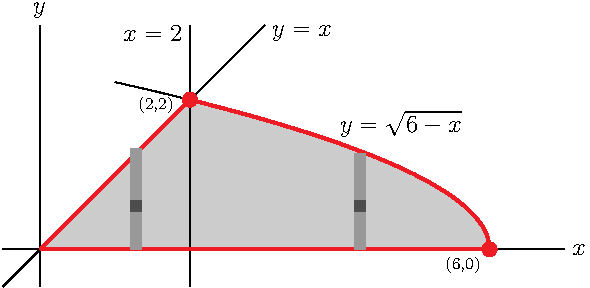
\includegraphics{OE14A_6.pdf}
\end{center}

To exchange the order of integration, we use horizontal slices as in the
figure below.

\begin{center}
     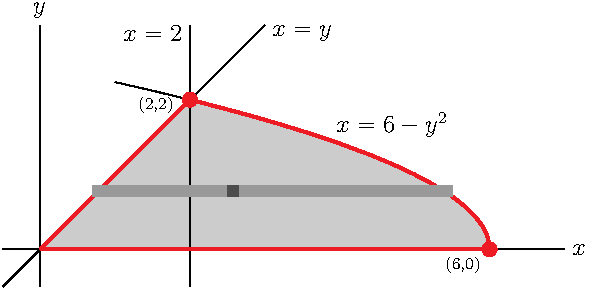
\includegraphics{OE14A_6h.pdf}
\end{center}

The bottom slice has $y=0$ and the top slice has $y=2$.
On the slice at height $y$, $x$ runs from $y$ to $6-y^2$. So
\begin{equation*}
I = \int_0^2 \int_y^{6-y^2} f(x,y)\ \dee{x}\,\dee{y}
\end{equation*}
\end{solution}

%%%%%%%%%%%%%%%%%%%%%%%%%%%%%%%%
\begin{question}[M200 2015D] %6
Consider the domain $D$ above the $x$--axis and below parabola 
$y = 1-x^2$ in the $xy$--plane.
\begin{enumerate}[(a)]
\item
Sketch $D$.
\item
Express
\begin{equation*}
\dblInt_D f(x,y)\ \dee{A}
\end{equation*}
as an iterated integral corresponding to the order $\dee{x}\,\dee{y}$. 
Then express this integral as an iterated integral corresponding to 
the order $\dee{y}\,\dee{x}$.
\item
Compute the integral in the case $f(x,y) = e^{x-(x^3/3)}$.
\end{enumerate}
\end{question}

%\begin{hint}
%
%\end{hint}

\begin{answer}
(a)

\begin{center}
\includegraphics{OE15D_6.pdf}
\end{center}


(b) $\int_0^1 \int_{-\sqrt{1-y}}^{\sqrt{1-y}} f(x,y)\ \dee{x}\,\dee{y}$,
    $\int_{-1}^1 \int_0^{1-x^2} f(x,y)\ \dee{y}\,\dee{x}$

(c) $e^{2/3}-e^{-2/3}$
\end{answer}

\begin{solution}
(a), (b) 
Looking at the figure on the left below, we see that we can write
the domain
\begin{equation*}
D = \Set{(x,y)}{0\le y\le 1,\ -\sqrt{1-y}\le x\le\sqrt{1-y}}
\end{equation*}
So
\begin{equation*}
\dblInt_D f(x,y)\ \dee{A}
=\int_0^1\dee{y} \int_{-\sqrt{1-y}}^{\sqrt{1-y}}\dee{x}\ f(x,y)
=\int_0^1 \int_{-\sqrt{1-y}}^{\sqrt{1-y}} f(x,y)\ \dee{x}\,\dee{y}
\end{equation*}

\begin{center}
\includegraphics{OE15D_6B.pdf}\qquad
\includegraphics{OE15D_6A.pdf}
\end{center}

Looking at the figure on the right above, we see that we can write
the domain
\begin{equation*}
D = \Set{(x,y)}{-1\le x\le 1,\ 0\le y\le 1-x^2}
\end{equation*}
So
\begin{equation*}
\dblInt_D f(x,y)\ \dee{A}
=\int_{-1}^1\dee{x} \int_0^{1-x^2}\dee{y}\ f(x,y)
=\int_{-1}^1 \int_0^{1-x^2} f(x,y)\ \dee{y}\,\dee{x}
\end{equation*}

(c) Using the second form from part (b),
\begin{align*}
\dblInt_D e^{x-(x^3/3)}\ \dee{A}
&=\int_{-1}^1\dee{x} \int_0^{1-x^2}\dee{y}\ e^{x-(x^3/3)} \\
&=\int_{-1}^1 (1-x^2) e^{x-(x^3/3)}\ \dee{x} \\
&=\int_{-2/3}^{2/3} e^u\ \dee{u} \qquad\text{with }
   u=x -\frac{x^3}{3},\ 
   \dee{u} = \big(1-x^2)\,\dee{x} \\
&= e^{2/3}-e^{-2/3}
\end{align*}
\end{solution}

%%%%%%%%%%%%%%%%%%%%%%%%%%%%%%%%
\begin{question}[M200 2016D] %6
Let $I=\int_0^1 \int_{x^2}^1 x^3\ \sin(y^3)\ \dee{y}\ \dee{x}$.
\begin{enumerate}[(a)]
\item
Sketch the region of integration in the $xy$--plane. Label your
sketch sufficiently well that one could use it to determine the
limits of double integration.

\item
Evaluate $I$.

\end{enumerate}
\end{question}

\begin{hint}
The inside integral, over $y$, looks pretty nasty
because $\sin(y^3)$ does not have an obvious antiderivative. So try
reversing the order of integration.
\end{hint}

\begin{answer}
(a)
\begin{center}
     \includegraphics{OE16D_6.pdf} 
\end{center}
(b) $\frac{1-\cos(1)}{12}$
\end{answer}

\begin{solution}
 (a) 
On the domain of integration,
\begin{itemize}
\item
$x$ runs from $0$ to $1$ and
\item 
for each fixed $x$ in that range, $y$ runs from $x^2$ to $1$.
\end{itemize}
The figure on the left below is a sketch of that domain, together with 
a generic vertical strip as was used in setting up the integral.

\begin{center}
     \includegraphics{OE16D_6v.pdf} \qquad
     \includegraphics{OE16D_6h.pdf} 
\end{center}

(b) As it stands, the inside integral, over $y$, looks pretty nasty
because $\sin(y^3)$ does not have an obvious antiderivative. So let's
reverse the order of integration. The given integral was set up 
using vertical strips. So, to reverse the order of integration, we use
horizontal strips as in the figure on the right above. Looking at that
figure we see that, on the domain of integration,
\begin{itemize}
\item
$y$ runs from $0$ to $1$ and
\item 
for each fixed $y$ in that range, $x$ runs from $0$ to $\sqrt{y}$.
\end{itemize}
So
\begin{align*}
I&=\int_0^1\dee{y} \int_0^{\sqrt{y}}\dee{x}\  x^3\ \sin(y^3) \\
 &=\int_0^1\dee{y}\ \sin(y^3)\left[\frac{x^4}{4}\right]_0^{\sqrt{y}} \\
 &=\frac{1}{4}\int_0^1\dee{y}\ y^2\sin(y^3) \\
 &=\frac{1}{4}\left[-\frac{\cos(y^3)}{3}\right]_0^1 \\
 &=\frac{1-\cos(1)}{12}
\end{align*}
\end{solution}

%%%%%%%%%%%%%%%%%%%%%%%%%%%%%%%%
\begin{question}[M200 2003D] %6
Consider the solid under the surface $z=6-xy$, bounded by
the five planes $x=0$, $x=3$, $y=0$, $y=3$, $z=0$. Note that no part of
the solid lies below the $x$--$y$ plane.
\begin{enumerate}[(a)]
\item
Sketch the base of the solid in the $xy$--plane. Note that
it is \emph{not} a square!
\item
Compute the volume of the solid.
\end{enumerate}
\end{question}

%\begin{hint}
%\end{hint}

\begin{answer}
(a)
\begin{center}
     \includegraphics{OE03DQ6a.pdf}
\end{center}

(b)
$27+18\ln\frac{3}{2}\approx 34.30$
\end{answer}

\begin{solution}
(a) The solid is the set of all $(x,y,z)$ obeying
$0\le x\le 3$, $0\le y\le 3$ and $0\le z\le 6-xy$. The base of this region
is the set of all $(x,y)$ for which there is a $z$ such that $(x,y,z)$
is in the solid. So the base is the set of all $(x,y)$ obeying
$0\le x\le 3$, $0\le y\le 3$ and $6-xy\ge 0$, i.e. $xy\le 6$. 
This region is sketched in the figure on the left below.

\begin{center}
     \includegraphics{OE03DQ6a.pdf} \qquad
     \includegraphics{OE03DQ6.pdf} 
\end{center}

(b) We'll deompose the base region into vertical strips as in the
figure on the right above.
Observe that the line $y=3$ intersects the curve $xy=6$ at the point $(2,3)$
and that on the base
\begin{itemize}
\item
$x$ runs from $0$ to $3$ and that
\item
for each fixed $x$ between $0$ and $2$, $y$ runs from $0$ to $3$, while
\item
for each fixed $x$ between $2$ and $3$, $y$ runs from $0$ to $6/x$
\end{itemize}
and that, for each $(x,y)$ in the base, $z$ runs from $0$ to $6-xy$.
So the 
\begin{align*}
\text{Volume}&=\int_0^2\dee{x}\int_0^3\dee{y}\ (6-xy)+
             \int_2^3\dee{x}\int_0^{6/x} \dee{y}\ (6-xy) \\
&=\int_0^2\dee{x}\ \left[6y-\frac{1}{2} xy^2\right]_0^3
+\int_2^3\dee{x}\ \left[6y-\frac{1}{2} xy^2\right]_0^{6/x} \\
&=\int_0^2\dee{x}\ \left[18-\frac{9}{2}x\right]
+\int_2^3\dee{x}\ \left[\frac{36}{x}-\frac{18}{x}\right] \\
&=\left[18x-\frac{9}{4}x^2\right]_0^2+\Big[18\ln x\Big]_2^3
=27+18\ln\frac{3}{2}\approx 34.30
\end{align*}
\end{solution}

%%%%%%%%%%%%%%%%%%%%%%%%%%%%%%%%
\begin{question}[M200 2002D] %6
Evaluate the following integral:
\begin{equation*}
\int_{-2}^2\int_{x^2}^4\cos\big(y^{3/2}\big)\ \dee{y}\,\dee{x}
\end{equation*}
\end{question}

\begin{hint}
The inside integral, $\int_{x^2}^4\cos\big(y^{3/2}\big)\ \dee{y}$,
in the given integral looks really nasty.  So try exchanging
the order of integration.
\end{hint}

\begin{answer}
$\frac{4}{3}\sin 8\approx 1.319$
\end{answer}

\begin{solution}
In the given integral
\begin{itemize}
\item 
$x$ runs from $-2$ to $2$ and
\item
for each fixed $x$ between $-2$ and $2$, $y$ runs from $x^2$ to $4$
\end{itemize}
So the domain of integration is 
\begin{equation*}
D = \Set{(x,y)}{-2\le x\le 2,\  x^2\le y\le 4}
\end{equation*}
This is sketched below. 
\begin{center}
     \includegraphics{OE02DQ6.pdf}
\end{center}
The inside integral, $\int_{x^2}^4\cos\big(y^{3/2}\big)\ \dee{y}$,
in the given integral looks really nasty.  So let's try exchanging
the order of integration. The given integral was formed by decomposing
the domain of integration $D$ into horizontal strips, like the blue strip
in the figure above. To exchange the order of integration we instead
decompose the domain of integration $D$ into vertical strips, 
like the pink strip in the figure above. To do so, we observe that, on $D$,
\begin{itemize}
\item 
$y$ runs from $0$ to $4$ and
\item
for each fixed $y$ between $0$ and $4$, $x$ runs from $-\sqrt{y}$ to $\sqrt{y}$.
\end{itemize}
That is, we reexpress the domain of integration as 
\begin{equation*}
D = \Set{(x,y)}{0\le y\le 4,\  -\sqrt{y}\le x\le \sqrt{y}}
\end{equation*}
and the given integral as
\begin{align*}
\int_{-2}^2\int_{x^2}^4\cos\big(y^{3/2}\big)\ \dee{y}\,\dee{x}
&=\int_0^4\dee{y} \int_{-\sqrt{y}}^{\sqrt{y}}\dee{x}\ \cos\big(y^{3/2}\big)\cr
&=\int_0^4\dee{y} \ 2\sqrt{y}\cos\big(y^{3/2}\big)\cr
&=\frac{4}{3}\int_0^8\dee{t}\ \cos t\quad\hbox{where }
    t=y^{3/2},\ \dee{t}=\frac{3}{2}\sqrt{y}\ \dee{y}\cr
&=\frac{4}{3}\sin t\Big|_0^8
=\frac{4}{3}\sin 8\approx 1.319
\end{align*}
\end{solution}

%%%%%%%%%%%%%%%%%%%%%%%%%%%%%%%%
\begin{question}[M200 2002A] %7
Consider the volume above the $xy$-plane that is inside
the circular cylinder $x^2+y^2=2y$ and underneath the surface $z=8+2xy$.
\begin{enumerate}[(a)]
\item
 Express this volume as a double integral $I$, stating clearly
the domain over which I is to be taken.

\item 
Express in Cartesian coordinates, the double integral $I$
as an iterated intergal in two different ways, indicating clearly the limits
of integration in each case.

\item
How much is this volume?
\end{enumerate}
\end{question}

%\begin{hint}
%\end{hint}

\begin{answer}
(a) $\dst I=\dblInt_D (8+2xy)\ \dee{x}\dee{y}$ where 
    $D=\Set{(x,y)}{x^2+(y-1)^2\le 1}$

(b) $\dst I
  =\int_0^2 \dee{y}\int_{-\sqrt{2y-y^2}}^{\sqrt{2y-y^2}}\dee{x}\ (8+2xy) 
  =\int_{-1}^1 \dee{x}\int_{1-\sqrt{1-x^2}}^{1+\sqrt{1-x^2}}\dee{y}\ (8+2xy)$

(c) $8\pi$
\end{answer}

\begin{solution}
(a) We may rewrite the equation $x^2+y^2=2y$ of the cylinder as
$x^2+(y-1)^2=1$. We are (in part (c)) to find the volume of the set
\begin{equation*}
V=\Set{(x,y,z)}{x^2+(y-1)^2\le 1,\ 0\le z\le 8+2xy}
\end{equation*}
When we look at this solid from far above (so that we can't see $z$) 
we see the set of points $(x,y)$ that 
obey $x^2+(y-1)^2\le 1$ and $8+2xy\ge 0$ (so that there is at least one allowed $z$ for that $(x,y)$). All points in $x^2+(y-1)^2\le 1$
have $-1\le x\le 1$ and $0\le y\le 2$ and hence $-2\le xy\le 2$ and
$8+2xy\ge 0$. So the domain of integration consists of the full disk
\begin{equation*}
D = \Set{(x,y)}{x^2+(y-1)^2\le 1}
\end{equation*}
The volume is 
\begin{equation*}
I=\dblInt_D (8+2xy)\ \dee{x}\dee{y}
\end{equation*}

(b)
We can express the double integral over $D$ as iterated integrals by
decomposing $D$ into horizontal strips, like the pink strip in the 
figure below, and also by decomposing $D$ into blue strips, like the 
blue strip in the figure below.
\begin{center}
     \includegraphics{OE02AQ7.pdf} 
\end{center}
For horizontal strips, we use that, on $D$
\begin{itemize}
\item
$y$ runs from $0$ to $2$ and,
\item
for each fixed $y$ between $0$ and $2$, $x$ runs from $-\sqrt{2y-y^2}$
to $\sqrt{2y-y^2}$ 
\end{itemize}
so that
\begin{equation*}
D=\Set{(x,y)}{0\le y\le 2,\ -\sqrt{2y-y^2}\le x\le \sqrt{2y-y^2}}
\end{equation*}
For vertical strips, we use that, on $D$
\begin{itemize}
\item
$x$ runs from $-1$ to $1$ and,
\item
for each fixed $x$ between $-1$ and $1$, $y$ runs from $1-\sqrt{1-x^2}$
to $1+\sqrt{1-x^2}$ 
\end{itemize}
so that
\begin{equation*}
D=\Set{(x,y)}{-1\le x\le 1,\ 1-\sqrt{1-x^2}\le x\le 1+\sqrt{1-x^2}}
\end{equation*}
Thus
\begin{align*}
I&=\int_0^2 \dee{y}\int_{-\sqrt{2y-y^2}}^{\sqrt{2y-y^2}}\dee{x}\ (8+2xy) \\
 &=\int_{-1}^1 \dee{x}\int_{1-\sqrt{1-x^2}}^{1+\sqrt{1-x^2}}\dee{y}\ (8+2xy)
\end{align*}

(c) Since $\dblInt_D 8\ \dee{x}\dee{y}$ is just $8$ times the area of $D$,
which is $\pi$,
\begin{align*}
\text{Volume}&=8\pi+\int_0^2 \dee{y}\int_{-\sqrt{2y-y^2}}^{\sqrt{2y-y^2}}\dee{x}\ 2xy
=8\pi+2\int_0^2 \dee{y}\ y\int_{-\sqrt{2y-y^2}}^{\sqrt{2y-y^2}}\dee{x}\ x \\
&=8\pi
\end{align*}
because $\int_{-\sqrt{2y-y^2}}^{\sqrt{2y-y^2}}\dee{x}\ x=0$ for all $y$,
because the integrand is odd and the domain of integration is even.
\end{solution}

%%%%%%%%%%%%%%%%%%%%%%%%%%%%%%%%
\begin{question}[M200 2001D] %6
Evaluate the following integral:
\begin{equation*}
\int_0^9\int_{\sqrt{y}}^3\sin(\pi x^3)\ \dee{x}\dee{y}
\end{equation*}
\end{question}

\begin{hint}
The inside integral, $\dst\int_{\sqrt{y}}^3\sin\big(\pi x^3\big)\ \dee{x}$,
in the given integral looks really nasty.  So try exchanging
the order of integration.
\end{hint}

\begin{answer}
$\frac{2}{3\pi}\approx 0.212$
\end{answer}

\begin{solution}
In the given integral
\begin{itemize}
\item 
$y$ runs from $0$ to $9$ and
\item
for each fixed $y$ between $0$ and $9$, $x$ runs from $\sqrt{y}$ to $3$
\end{itemize}
So the domain of integration is 
\begin{equation*}
D = \Set{(x,y)}{0\le y\le 9,\  \sqrt{y}\le x\le 3}
\end{equation*}
This is sketched below. 
\begin{center}
     \includegraphics{OE01DQ6.pdf}
\end{center}
The inside integral, $\int_{\sqrt{y}}^3\sin\big(\pi x^3\big)\ \dee{x}$,
in the given integral looks really nasty.  So let's try exchanging
the order of integration. The given integral was formed by decomposing
the domain of integration $D$ into horizontal strips, like the blue strip
in the figure above. To exchange the order of integration we instead
decompose the domain of integration $D$ into vertical strips, 
like the pink strip in the figure above. To do so, we observe that, on $D$,
\begin{itemize}
\item 
$x$ runs from $0$ to $3$ and
\item
for each fixed $x$ between $0$ and $3$, $y$ runs from $0$ to $x^2$.
\end{itemize}
That is, we reexpress the domain of integration as 
\begin{equation*}
D = \Set{(x,y)}{0\le x\le 3,\  0\le y\le x^2}
\end{equation*}
and the given integral as
\begin{align*}
\int_0^9\int_{\sqrt{y}}^3\sin(\pi x^3)\ \dee{x}\dee{y}
&=\int_0^3\dee{x} \int_0^{x^2}\dee{y}\ \sin(\pi x^3) \cr
&=\int_0^3\dee{x} \ x^2\sin(\pi x^3)\cr
&=\frac{1}{3\pi}\int_0^{27\pi}\dee{t}\ \sin t\quad\hbox{where }
    t=\pi x^3,\ \dee{t}=3\pi x^2\,\dee{x}\cr
&=-\frac{1}{3\pi}\cos t\Big|_0^{27\pi}=-\frac{1}{3\pi}\cos t\Big|_0^\pi
=\frac{2}{3\pi}\approx 0.212
\end{align*}
\end{solution}

%%%%%%%%%%%%%%%%%%%%%%%%%%%%%%%%
\begin{question}[M200 2000D] %6
The iterated integral
\begin{equation*}
I=\int_0^1\bigg[\int_{-\sqrt{x}}^{\sqrt{x}} \sin\big(y^3-3y\big)\,\dee{y}\bigg]
         \ \dee{x}
\end{equation*}
is equal to $\dblInt_R\sin\big(y^3-3y)\ dA$ for a suitable region $R$ in
the $xy$-plane.
\begin{enumerate}[(a)]
\item
Sketch the region $R$.

\item 
Write the integral $I$ with the orders of integration reversed,
and with suitable limits of integration.

\item 
Find $I$.
\end{enumerate}
\end{question}

%\begin{hint}
%
%\end{hint}

\begin{answer}

(b) $\dst\int_{-1}^1\bigg[\int_{y^2}^1 \sin\big(y^3-3y\big)\,\dee{x}\bigg]\ \dee{y}$
\qquad (c) $0$
\end{answer}

\begin{solution}
(a) In the given integral
\begin{itemize}
\item
$x$ runs from $0$ to $1$, and
\item
for each fixed $x$ between $0$ and $1$,
$y$ runs from $-\sqrt{x}$ to $\sqrt{x}$.
\end{itemize}
So the region
\begin{equation*}
R=\Set{(x,y)}{0\le x\le 1,\ -\sqrt{x}\le y\le \sqrt{x}}
\end{equation*}
It is sketched below.
\begin{center}
     \includegraphics{OE00DQ6.pdf}
\end{center}

(b) The given integral was formed by decomposing
the domain of integration $R$ into vertical strips, like the pink strip
in the figure above. To exchange the order of integration we instead
decompose the domain of integration $R$ into horizontal strips, 
like the blue strip in the figure above. To do so, we observe that, on $R$,
\begin{itemize}
\item 
$y$ runs from $-1$ to $1$, and
\item
for each fixed $y$ between $-1$ and $1$, $x$ runs from $y^2$ to $1$.
\end{itemize}
So 
\begin{equation*}
I=\int_{-1}^1\bigg[\int_{y^2}^1 \sin\big(y^3-3y\big)\,\dee{x}\bigg]\ \dee{y}
\end{equation*}

(c) The easy way to evaluate $I$ is to observe that, since 
$\sin\big(y^3-3y\big)$ is odd under $y\rightarrow -y$, the integral
\begin{equation*}
\int_{-\sqrt{x}}^{\sqrt{x}} \sin\big(y^3-3y\big)\,\dee{y}=0
\end{equation*}
for all $x$. Hence $I=0$. The hard way is 
\begin{align*}
I&=\int_{-1}^1\bigg[\int_{y^2}^1 \sin\big(y^3-3y\big)\,\dee{x}\bigg]\ \dee{y}\\
&=\int_{-1}^1 (1-y^2) \sin\big(y^3-3y\big)\ \dee{y}\\
&=\int_2^{-2} \sin t\ \frac{\dee{t}}{-3}
\qquad\hbox{ where }t=y^3-3y,\ \dee{t} =3(y^2-1)\,\dee{y} \\
&=\frac{1}{3}\cos t\ \Big|_2^{-2}=0
\end{align*}
again, since $\cos$ is even.
\end{solution}

%%%%%%%%%%%%%%%%%%%%%%%%%%%%%%%%
\begin{question}[M200 2000A] %7
Find the double integral of the function $f(x, y) = xy$
 over the region bounded by $y = x - 1$ and $y^2 = 2x + 6$.
\end{question}

%\begin{hint}
%
%\end{hint}

\begin{answer}
$36$
\end{answer}

\begin{solution}
The parabola $y^2=2x+6$ and the line $y=x-1$ meet when $x=y+1$
with $y^2=2(y+1)+6$ or $y^2-2y-8=(y-4)(y+2)=0$. So they meet at $(-1,-2)$ and $(5,4)$.
The domain of integration is sketched below. 
\begin{center}
     \includegraphics{OE00AQ7.pdf}
\end{center}
On this domain
\begin{itemize}
\item
$y$ runs from $-2$ to $4$, and
\item
for each fixed $y$ between $-2$ and $4$, $x$ runs from $\frac{y^2}{2}-3$
to $y+1$.
\end{itemize}
So the integral is 
\begin{align*}
\int_{-2}^4\dee{y}\int_{y^2/2-3}^{y+1}\dee{x}\ xy
&=\int_{-2}^4\dee{y}\ \frac{1}{2} x^2y\bigg|_{y^2/2-3}^{y+1} \\
&=\frac{1}{2}\int_{-2}^4\dee{y}\ 
                  \left[y^3+2y^2+y-\frac{1}{4}y^5+3y^3-9y\right] \\
&=\frac{1}{2}\int_{-2}^4\dee{y}\ \left[-8y+2y^2+4y^3-\frac{1}{4}y^5\right] \\
&=\left[-2y^2+\frac{1}{3}y^3+\frac{1}{2}y^4-\frac{1}{48}y^6\right]_{-2}^4 \\
&=-2(16-4)+\frac{1}{3}(64+8)+\frac{1}{2}(256-16)
-\frac{1}{48}(4096-64)\cr
&=-24+24+120-84=36
\end{align*}
\end{solution}



%%%%%%%%%%%%%%%%%%
\subsection*{\Application}
%%%%%%%%%%%%%%%%%%

%%%%%%%%%%%%%%%%%%%%%%%%%%%%%%%%
\begin{question}
Find the volume of the solid inside the cylinder $x^2+2y^2=8$, above
the plane $z=y-4$ and below the plane $z=8-x$.
\end{question}

%\begin{hint}
%
%\end{hint}

\begin{answer}
$48\sqrt{2}\,\pi$
\end{answer}

\begin{solution}
Looking down from the top, we see the cylinder 
$x^2+2y^2\le 8$. That gives the base region. The top of the solid, above
any fixed $(x,y)$ in the base region, is at $z=8-x$ (this is always positive
because $x$ never gets bigger than $\sqrt{8}$) . The bottom 
of the solid, below any fixed $(x,y)$ in the base region, is at 
$z=y-4$ (this is always negative because $y$ is always smaller than $2$).
So the height of the solid at any $(x,y)$ is 
\begin{equation*}
z_{\rm top}-z_{\rm bottom}
=(8-x)-(y-4)=12-x-y
\end{equation*} 
The volume is
\begin{equation*}
\int_{-2}^{2}\dee{y}\int_{-\sqrt{8-2y^2}}^{\sqrt{8-2y^2}}\dee{x}\ (12-x-y)
\end{equation*}
Recall, from Theorem \eref{CLP101}{thm:INTevenodd} in the CLP-2 text, 
that if $f(x)$ is an odd function (meaning that
$f(-x)=-f(x)$ for all $x$), then $\int_{-a}^a f(x)\ \dee{x}=0$ (because the 
two integrals $\int_0^a f(x)\ \dee{x}$ and $\int_{-a}^0 f(x)\ \dee{x}$ have the 
same magnitude but opposite signs). Applying this twice gives
\begin{equation*}
\int_{-\sqrt{8-2y^2}}^{\sqrt{8-2y^2}}\dee{x}\ x=0\text{ and }
\int_{-2}^{2}\dee{y}\int_{-\sqrt{8-2y^2}}^{\sqrt{8-2y^2}}\dee{x}\ y
=\int_{-2}^{2}\dee{y}\ 2y\sqrt{8-2y^2}=0
\end{equation*}
since $x$ and $y\sqrt{8-2y^2}$ are both odd. Thus
\begin{equation*}
\int_{-2}^{2}\dee{y}\int_{-\sqrt{8-2y^2}}^{\sqrt{8-2y^2}}\dee{x}\ (-x-y)=0
\implies 
\text{Volume} = \int_{-2}^{2}\dee{y}\int_{-\sqrt{8-2y^2}}^{\sqrt{8-2y^2}}\dee{x}\ 
12
\end{equation*}
so that the volume is just 12 times the area of the ellipse $x^2+2y^2=8$,
which is
\begin{equation*}
12\big(\pi\,\sqrt{8}\,2\big)= 48\sqrt{2}\,\pi
\end{equation*}
\end{solution}